%%%%%%%%%%%%%%%%%%%%%%%%%%%%%%%%%%%%%%%%%%%%%%%%%%%%%%%%%%%%%%%%%%%%%%%%%%%%%%%
% Memorial para concurso público de Professor Doutor na USP.
%
% Formatação inspirada em:
% * https://tug.org/pracjourn/2008-1/mori/mori.pdf
% * https://github.com/santisoler/phd-thesis
% * https://github.com/compgeolab/dissertation-template
%%%%%%%%%%%%%%%%%%%%%%%%%%%%%%%%%%%%%%%%%%%%%%%%%%%%%%%%%%%%%%%%%%%%%%%%%%%%%%%

%%%%%%%%%%%%%%%%%%%%%%%%%%%%%%%%%%%%%%%%%%%%%%%%%%%%%%%%%%%%%%%%%%%%%%%%%%%%%%%
% Set a class and import packages
\documentclass[11pt,a4paper,oneside]{book}

\usepackage[utf8]{inputenc}
\usepackage[T1]{fontenc}
\usepackage[brazil]{babel}
\usepackage[width=150mm,top=40mm,bottom=30mm,headsep=10mm,headheight=5mm]{geometry}
\usepackage{graphicx}
\usepackage{amssymb}
\usepackage{amsmath}
\usepackage{hyperref}
% create fancy headers
\usepackage{fancyhdr}
% commands for managing dates and its formats
\usepackage{datetime2}
% improved urls with proper hyphenation
\usepackage{xurl}
% Import enumitem to customize descriptions in license.tex
\usepackage{enumitem}
% Make caption titles bold
\usepackage[labelfont=bf,font=small,skip=0pt]{caption}
% To control the style of section titles
\usepackage{titlesec}
% Add the bibliography to the table of contents
\usepackage[nottoc,chapter]{tocbibind}
\usepackage[round,authoryear,sort]{natbib}
% Use custom apalike bibliography style
\bibliographystyle{apalike-doi}
% show dois as links on references
\usepackage{doi}
% Icon fonts (requires using xelatex or luatex)
\usepackage[fixed]{fontawesome5}
\usepackage{academicons}
% Set fonts (requires compilation with xelatex)
\usepackage{fontspec}
%%%%%%%%%%%%%%%%%%%%%%%%%%%%%%%%%%%%%%%%%%%%%%%%%%%%%%%%%%%%%%%%%%%%%%%%%%%%%%%

%%%%%%%%%%%%%%%%%%%%%%%%%%%%%%%%%%%%%%%%%%%%%%%%%%%%%%%%%%%%%%%%%%%%%%%%%%%%%%%
% Configuration of the document

\setmainfont[%
  Path = fonts/notoserif/,
  UprightFont = NotoSerif-Regular,
  BoldFont = NotoSerif-Bold,
  ItalicFont = NotoSerif-Italic,
  Extension = .ttf
]{NotoSerif}

% Increase the line spacing
\renewcommand{\baselinestretch}{1.5}

% Customize how Chapter headings are displayed
\titleformat{\chapter}[display]{\normalfont}{}{5pt}{\vspace{-3.5cm}\huge}

% Variables
\newcommand{\Author}{%
  Leonardo Uieda
}
\newcommand{\Year}{%
  2022
}

% Configure hyperref and add PDF metadata
\hypersetup{
    colorlinks,
    allcolors=[rgb]{0, 0.451, 0.753},
    pdftitle={Memorial para concurso publico de Professor Doutor na USP},
    pdfauthor={\Author},
    pdftex,
}

% make urls use the same font as every other text
\urlstyle{same}

% Define emptypage command
\newcommand{\emptypage}{%
    \newpage
    \thispagestyle{empty}
    \mbox{}
    \newpage
}

% Configure headers and footers
\fancyhf{}
\lhead{\fontsize{10pt}{0}\selectfont\itshape \nouppercase\leftmark}
\chead{}
\rhead{\fontsize{9pt}{0}\selectfont \thepage}
\cfoot{}
\renewcommand{\headrulewidth}{0pt}
%%%%%%%%%%%%%%%%%%%%%%%%%%%%%%%%%%%%%%%%%%%%%%%%%%%%%%%%%%%%%%%%%%%%%%%%%%%%%%%

%%%%%%%%%%%%%%%%%%%%%%%%%%%%%%%%%%%%%%%%%%%%%%%%%%%%%%%%%%%%%%%%%%%%%%%%%%%%%%%
\begin{document}

\pagestyle{plain}
\frontmatter
%\fancyfront

\begin{titlepage}
  \begin{center}
    
\includegraphics[height=2cm]{images/logo.pdf}
    \vspace{1cm}

    MEMORIAL PARA CONCURSO PÚBLICO

    PROFESSOR DOUTOR (RDIDP) EM MÉTODOS POTENCIAIS

    UNIVERSIDADE DE SÃO PAULO
    \vspace{4cm}

    \textbf{\LARGE \MakeUppercase{\Author{}}}
    \vspace{5cm}

    {\small
      Apresentado para concurso público de títulos e provas para cargo de

      Professor Doutor junto ao Departamento de Geofísica do

      Instituto de Astronomia, Geofísica e Ciências Atmosféricas da

      Universidade de São Paulo.
      \vspace{1cm}

      Edital ATAc-IAG/044/2022
    }
    \vfill

    \Year{}
  \end{center}
\end{titlepage}

%==============================================================================
\chapter*{Resumo}

Resumo curto.
Quem eu sou.
Principais highlights.
Sobre esse memorial (organização etc).
Meu papel no IAG.
Grande parte do texto que está na introdução do memorial antigo.

%==============================================================================
\tableofcontents

\pagestyle{fancy}
\mainmatter

%==============================================================================
\chapter{Introdução}

Sobre meus pais e meu primeiro contato com a pesquisa e ensino superior.
A ética e dedicação eles me passaram.
A oportunidade de morar no exterior.

Disclaimer sobre meus privilégios.
O memorial é uma reflexão das minhas conquistas.
É importante refletir também nos privilégios que me permitiram chegar onde cheguei.
Nem tudo é mérito.
Suporte familiar.
Classe média e não tive que trabalhar para apoiar meus estudos.
Escola privada.
Oportunidade de morar fora e aprender inglês.
Brasil possui ensino superior gratuito e bolsas.
Ida para o Canada foi financiada pelos meus pais.
Muitas coisas sobre o dia a dia na academia eu já sabia por ver meus pais.
Estigma contra asiáticos é relativamente baixo, pode até ser positivo nas ciências exatas.
Sorte na escolha de curso, ano de ingresso, política a favor da ciência,
professores (Mary Lilian Lourenço, Manoel Roberto Robilotta, Alan Mitchell
Durham) e mentores (Manuel, Ricardo,
Naomi, Val, Carla, Paul), vagas na hora certa, confiança e suporte para reconhecer
opoturnidades e ir atrás.


\begin{figure}[h]
  \vspace{0.5cm}
  \begin{center}
    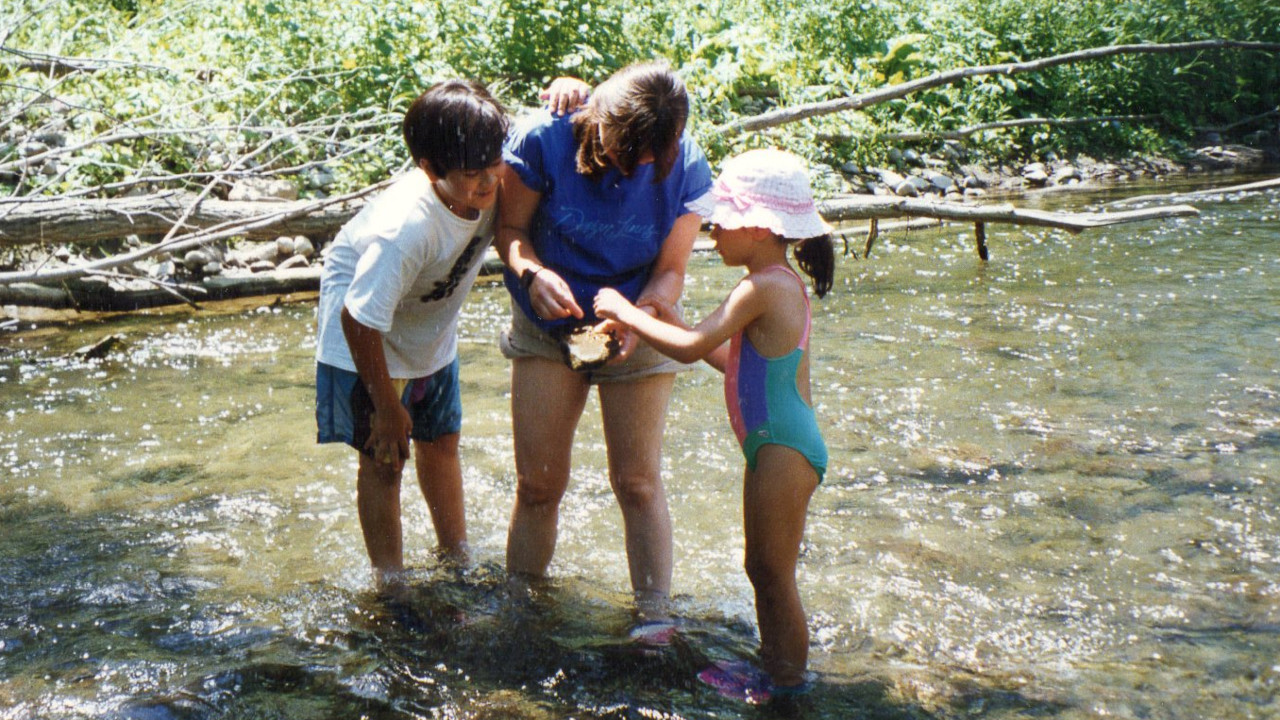
\includegraphics[width=\textwidth]{images/1997-06-ithaca-creek.jpg}
  \end{center}
  \caption{
    Bla
  }
\end{figure}

%==============================================================================
\chapter{Formação Acadêmica}

Começa de quando ingressei na USP.
Coisas que eu aprendi, IC, TCC, campos, etc.
Turma de graduação e como isso influenciou meu pensamento.
Intercâmbio em York, geodésia, e o
Spiros Pagiatakis\footnote{\url{https://www.yorku.ca/spiros/spiros.html}}.

\begin{figure}[h]
  \vspace{0.5cm}
  \begin{center}
    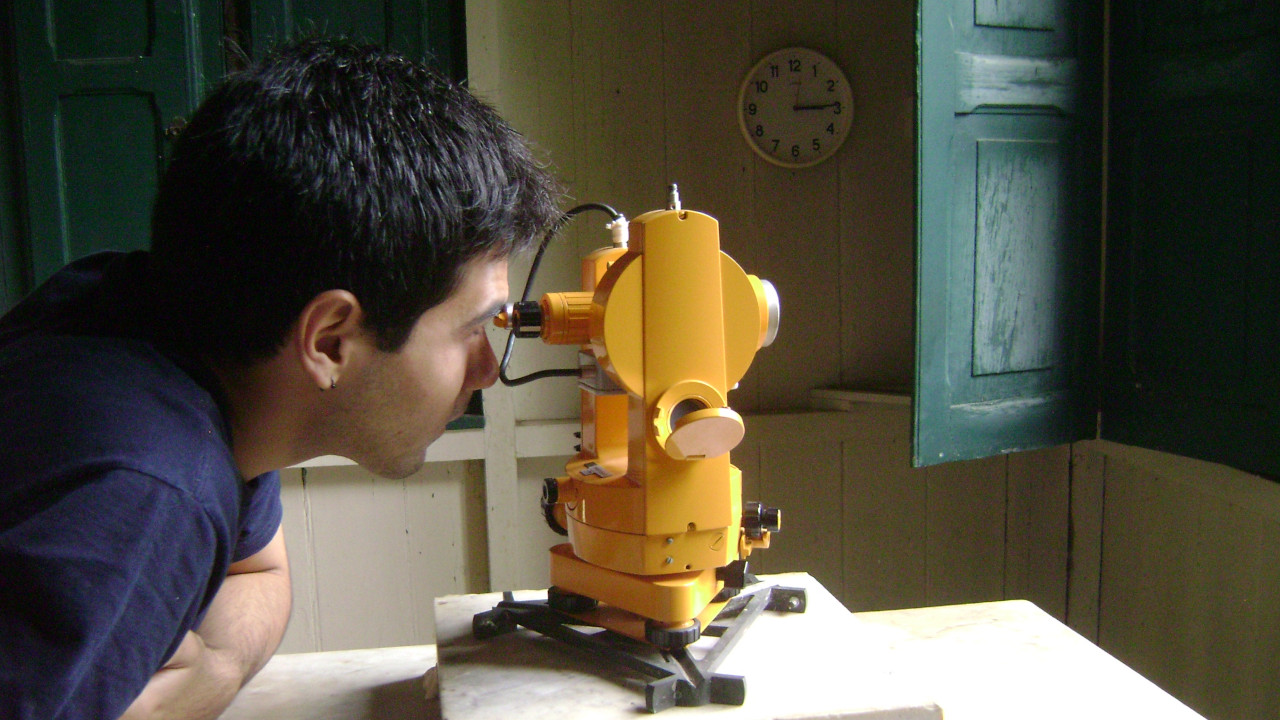
\includegraphics[width=\textwidth]{images/vassouras-geomag-observation-2012.jpg}
  \end{center}
  \caption{
    Bla
  }
\end{figure}

\begin{figure}[h]
  \vspace{0.5cm}
  \begin{center}
    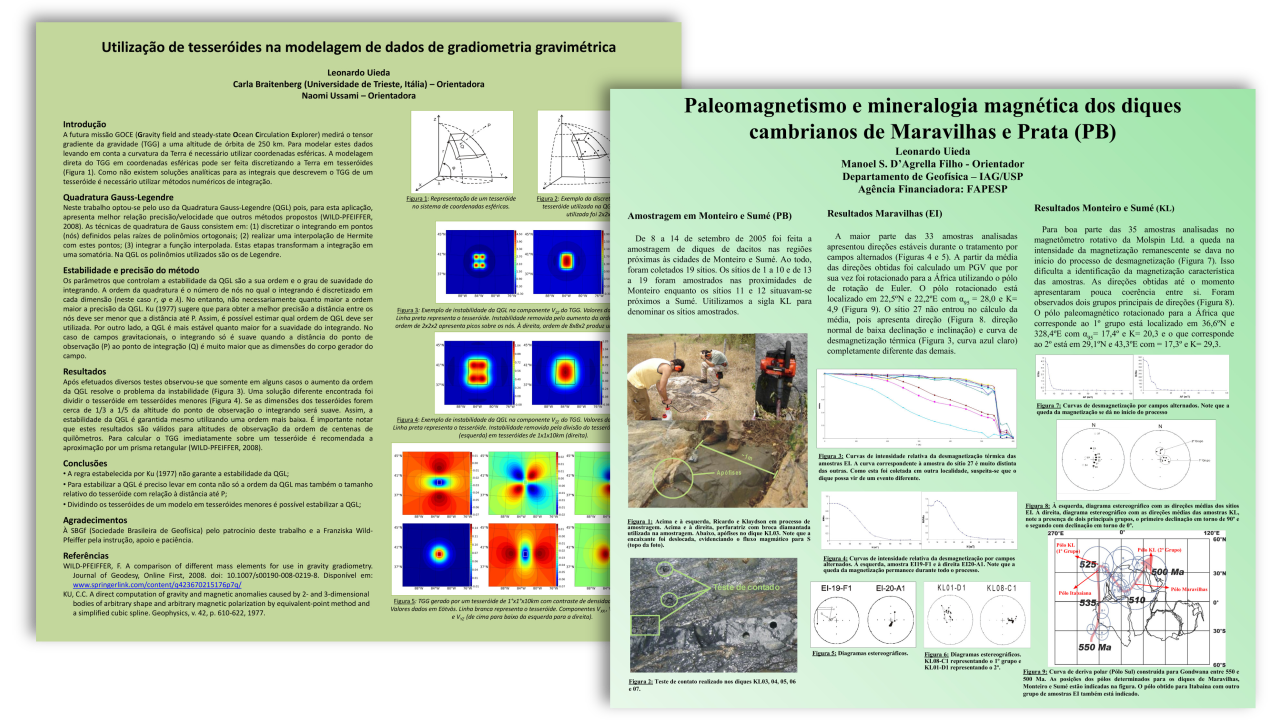
\includegraphics[width=\textwidth]{images/posters-iag.png}
  \end{center}
  \caption{
    Bla
  }
\end{figure}

%==============================================================================
\chapter{Linhas de Pesquisa}

\begin{figure}[h]
  \vspace{0.5cm}
  \begin{center}
    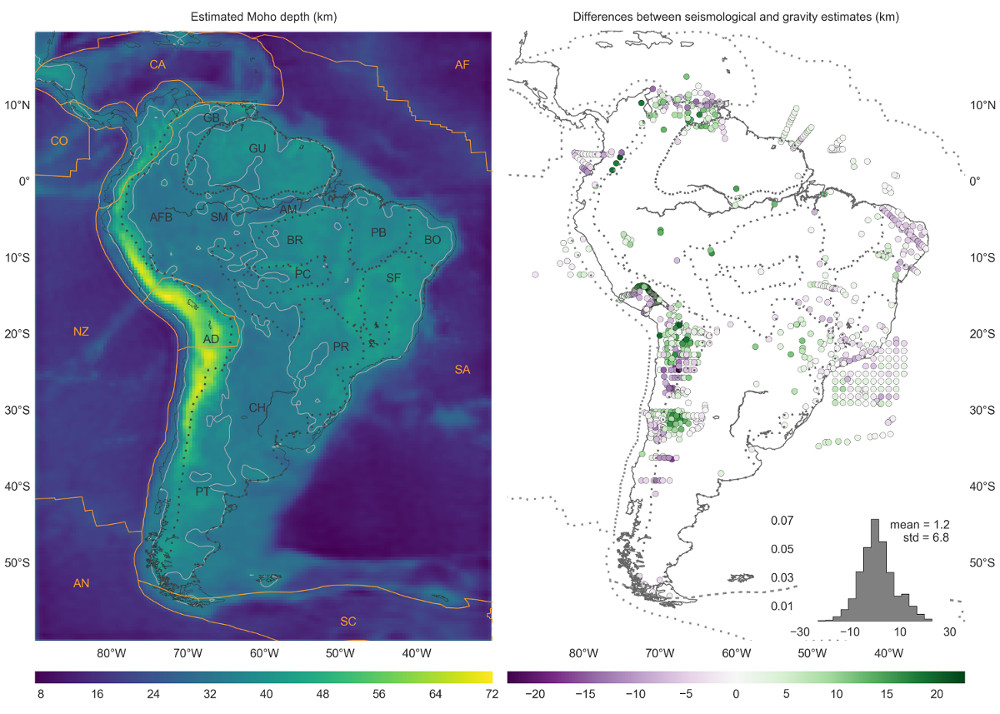
\includegraphics[width=\textwidth]{images/south-american-moho.jpg}
  \end{center}
  \caption{
    Bla
  }
\end{figure}

%==============================================================================
\chapter{Experiência em Ensino}

\begin{figure}[h]
  \vspace{0.5cm}
  \begin{center}
    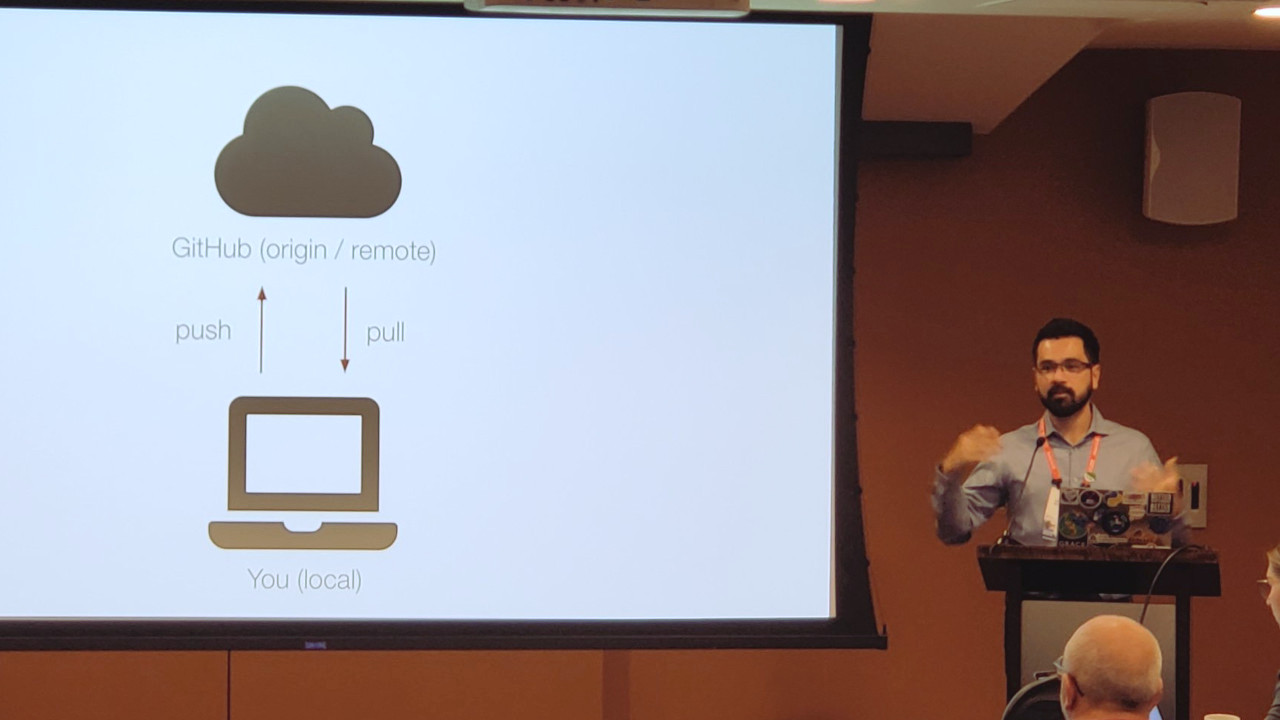
\includegraphics[width=\textwidth]{images/agu-2019-git-lesson.jpg}
  \end{center}
  \caption{
    Bla
  }
\end{figure}

Figura do notebook de ondas sísmicas.

\begin{figure}[h]
  \vspace{0.5cm}
  \begin{center}
    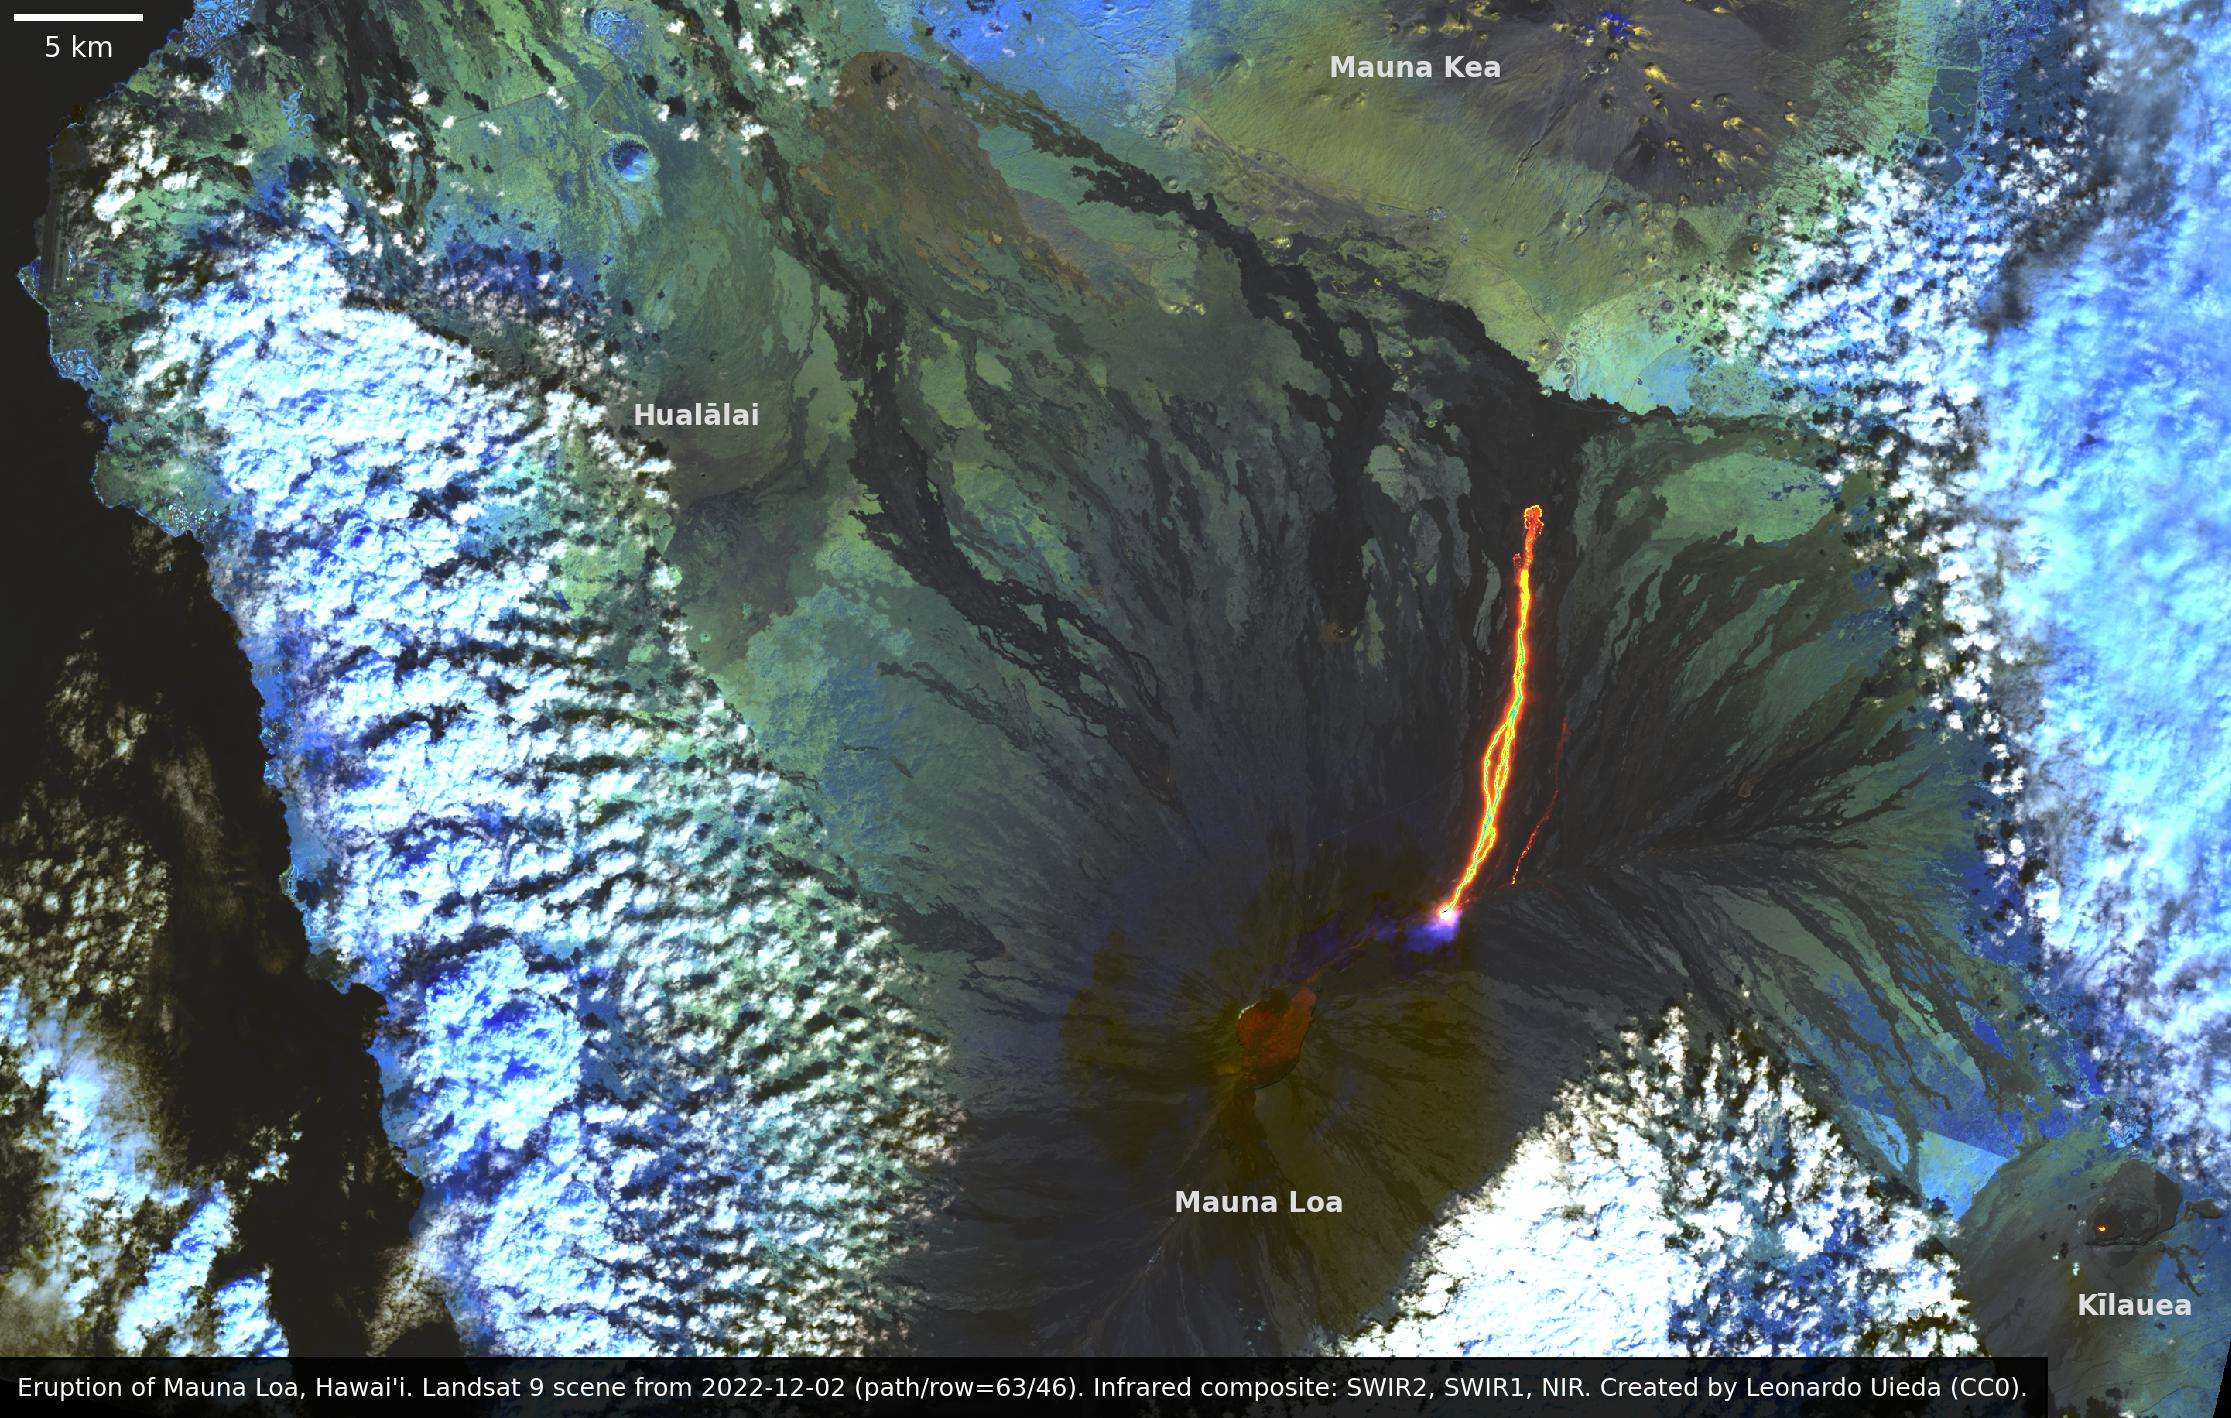
\includegraphics[width=\textwidth]{images/mauna-loa-landsat-2022-12-02.jpg}
  \end{center}
  \caption{
    Bla
  }
\end{figure}

%==============================================================================
\chapter{Ciência Aberta}


\begin{figure}[h]
  \vspace{0.5cm}
  \begin{center}
    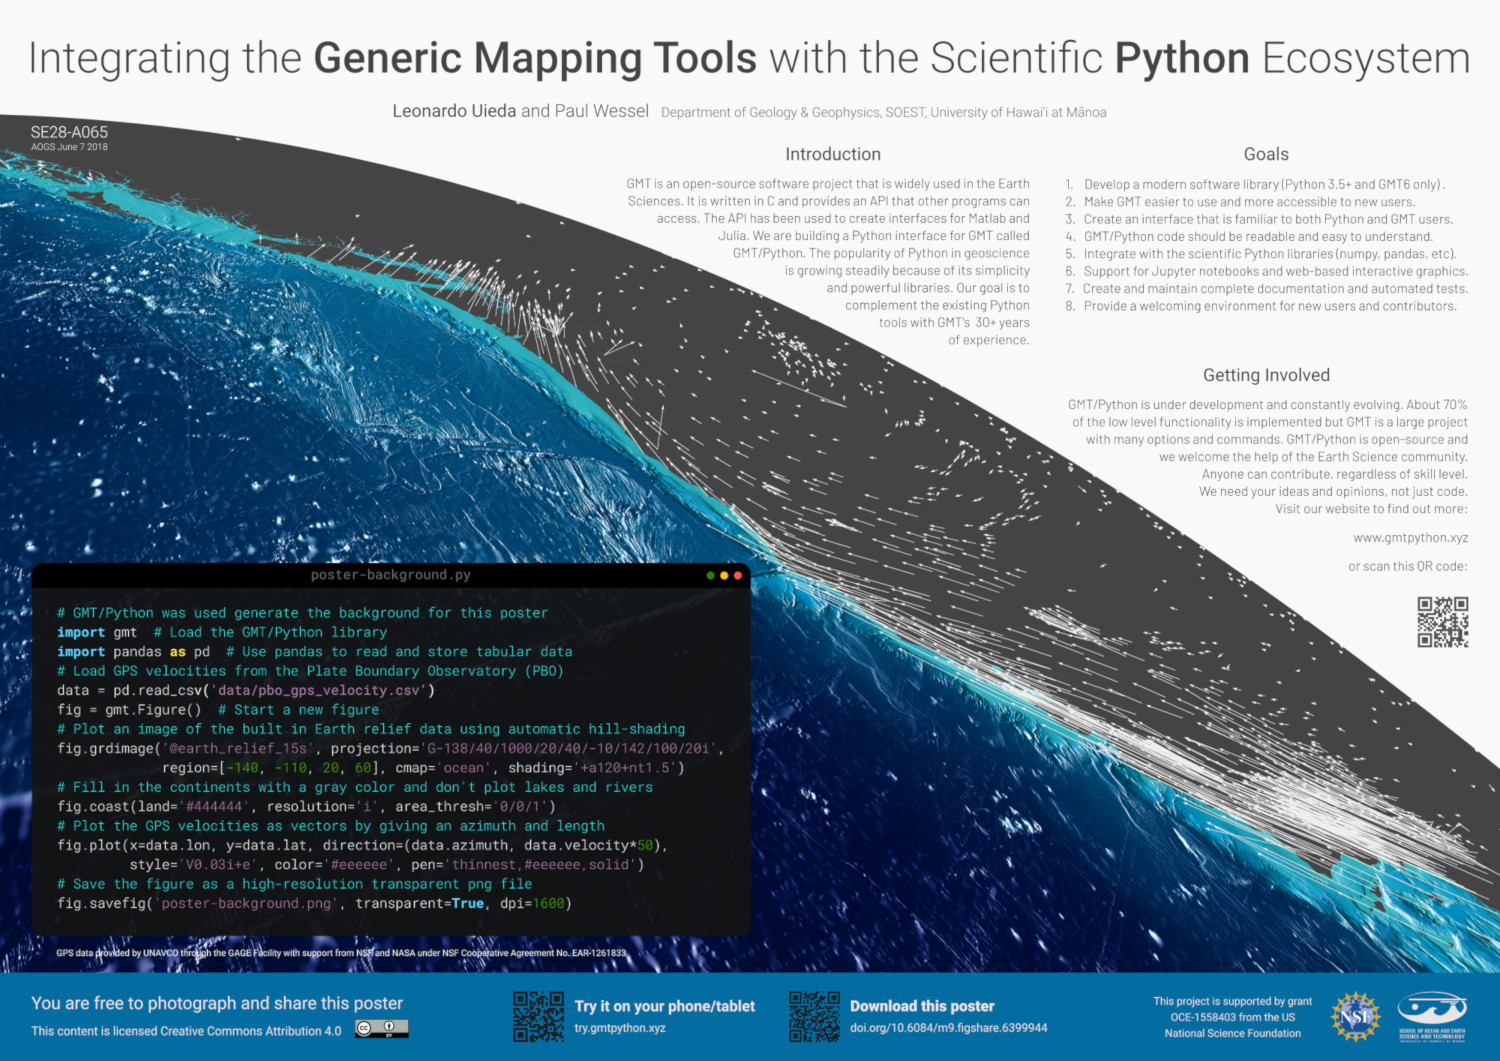
\includegraphics[width=\textwidth]{images/aogs2018.jpg}
  \end{center}
  \caption{
    Bla
  }
\end{figure}

%==============================================================================
\chapter{Conclusão}

Repete resumo dos principais pontos.
Termina com o que eu pretendo conquistar no futuro.

%==============================================================================
\backmatter
%\phantomsection  % use phantomsection to fix bibliography href in the toc
\bibliography{references}

\end{document}
